\documentclass[a4paper,12pt]{article}
\usepackage{color}
\usepackage{graphicx} %Needed to include pictures in the document.

\begin{document}

	\title{My First {\LaTeX} Document}
	\author{Jose Ángel Gumiel}
	\date{\today}
	\maketitle
	
	%With the percentage symbol, I can write comments on the code. This does not compile, so it does not show up in the generated pdf neither.
	
	\pagenumbering{roman}
	\tableofcontents
	\newpage
	\pagenumbering{arabic}
	
	\section{Introduction}
	I am going to test {\LaTeX} for the very first time.
	
	\section{Methods}
		\subsection{Stage 1}
		\label{sec1}
		The first part is installing TeXworks.
		
		\subsection{Stage 2}
		The second part is reading a tutorial.
		
		\subsection{Stage 3}
		This stage is dedicated to typesetting.\\
		\textit{Italic}, \textsl{slanted}, \textsc{ smallcaps}, CAPS, \textbf{bold}, \texttt{teletype}, \textsf{SansSerif}, \textrm{roman}, \underline{underlined}.\newline
		{\color{red}Fire.}\break
		\textbf{{\color{red}Fire.}} \break
		Now I am going to play with font sizes:
		{\tiny tiny words}, {\scriptsize scriptsize}, {\footnotesize footnotesize}, {\small small}, {\normalsize normalsize}, {\large large}, {\Large Large}, {\LARGE LARGE}, {\huge huge}.\\
		\\
		Let's recopile what I have done with an easy list.
		
		\begin{enumerate}
			\item Install TeXworks
			\item Read a tutorial
			\item Try and fail
			\begin{enumerate}
				\item Typesetting
				\item Colour
				\item Size
			\end{enumerate}
			\item Results
			\begin{itemize}
				\item Beautiful Document
				\item Some knowledge
			\end{itemize}
			\item More is to come.
		\end{enumerate}


		Let's create blankspaces: \\%SMTH IS BAD.
		S \hspace{10pt} P \hspace{40pt} A \hspace{60pt} C \hspace{80pt} E \\
		If you use vspace insted of hspace, it is vertical space.\\
		\\
		What about special characters? Then, insert an slash: \# \_ \%. Nice.\\
		Let's concatenate them: \# \& \%\\
		%An exercise is to write the following sentence: Item #1A\642 costs $8 & is sold at a  ̃10% profit.
		Item \#1A\textbackslash642 costs \$8 \& is sold at \~{}10\% profit.\\

		\subsection{Stage 4}
		This stage is dedicated to tables.\\
		\\
		\begin{tabular}{|l|c|r|}
			\hline
			Column 1 & Column 2 & Column 3\\
			\hline
			Left & Center & Right\\
			Izquierda & Centro & Derecha\\
			Sinistra & Centro & Destra\\
			Gauche & Centre & Droite\\
			\hline
		\end{tabular}
		\\\\\\\\ %Creating some lines
		\begin{tabular}{|l|l|}
			Apples & Green \\
			Strawberries & Red \\
			Oranges & Orange \\
		\end{tabular}
		\\\\\\\\
		\begin{tabular}{rc}
			Apples & Green \\
			\hline
			Strawberries & Red \\
			\cline{1-1}
			Oranges & Orange \\
		\end{tabular}
		\\\\\\\\
		\begin{tabular}{|r|l|}
			\hline
			8 & here’s \\
			\cline{2-2}
			86 & stuff \\
			\hline \hline
			2008 & now \\
			\hline
		\end{tabular}
		\\\\\\\\
		\begin{tabular}{l|r|r}
			Item & Quantity & Price  \(\$\)\\
			\hline
			Nails & 500 & 0.34\\
			Wooden boards & 100 & 4.00\\
			Bricks & 240 & 11.50\\
		\end{tabular}
		\\\\\\\\
		\begin{tabular}{l|ccc}
			 & & Year & \\
			\cline{2-4}
			City & 2006 & 2007 & 2008\\
			\hline
			London & 45789 & 46551 & 51298\\
			Berlin & 34549 & 32543 & 29870 \\
			Paris & 49835 & 51009 & 51970 \\
		\end{tabular}

		\subsection{Stage 5}
		What about illustrations? Sure I can add some fancy pictures here. \\\\
		Beware, graphicx package is needed!!!\\\\

		\begin{figure}[h]%h stands for place HERE. It looks for the best fitting.
			\centering
			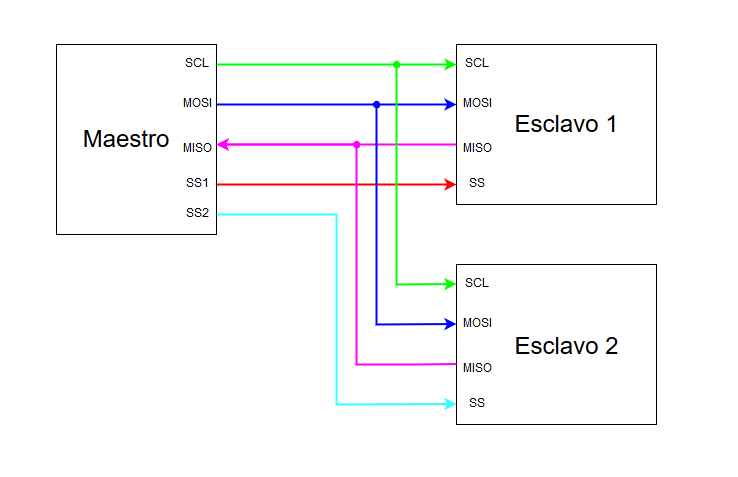
\includegraphics[width=1\textwidth]{Images/SPI-scheme.png}
			\caption{ This is a SPI protocol wiring scheme.}
		\end{figure}
		
		\subsection{Stage 6}
		Now I am doing some maths.


	\section{Results}
	Here are my results. Pretty text, uh?
	Now I am going to try referring section \ref{sec1} on page \pageref{sec1}

\end{document}